\renewcommand{\theauthor}{Dario Wagner}
\chapter{Technologien}
\label{sec:Technologien}
\section{Allgemeines}
\label{sec:TechnologieAllgemeines}
Die, während der Diplomarbeit, verwendeten Technologien werden anschließend, unter entsprechender Überschrift, beschrieben. Wobei auf die wichtigsten, oder auch meist benutzten, genauer eingegangen wird, in Form einer Installation und einer erweiterten Beschreibung. Zudem werden auch alle Technologien beschrieben welche sich nicht bis zum Ende der Arbeit durchsetzen konnten und während der Arbeit durch eine andere ersetzt wurden oder überhaupt nicht mehr verwendet wurden. Dies wird jedoch im Beschreibungstext kenntlich gemacht.
\section{Programmierung}
\label{sec:TechnologieProgrammierung}
Dieses Unterkapitel befasst sich mit allen Technologien welche im Laufe der Programmierung verwendet wurden. Alle programmier-bezogenene Technologien werden aufgelistet und je nach Wichtigkeit teilweise erklärt.
\subsubsection{C\#}
\label{sec:CSharp}
Der praktische Teil der Diplomarbeit wurde mithilfe der Objekt-Orientierten Programmiersprache C\# entwickelt, da die Firma Intact GmbH, der Auftraggeber der Diplomarbeit, in der C\#/.NET-Entwicklung tätig ist. \\ \break
C\# wurde im Jahr 2001 von Microsoft speziell für die .NET Umgebung veröffentlicht und ist daher eine junge Programmiersprache. C\# hat mehrere Anwendungsbereiche unter anderem können Desktopanwendungen, XML Web services, Datenbankanwendungen und vieles mehr entwickelt werden. \\ \break
Die ''geschwungene Klammer''-Syntax von C\# ist sehr ähnlich zu Java, C oder C++. Falls eine dieser Programmiersprachen bekannt ist, ist es einfach in kurzer Zeit zu lernen in C\# zu programmieren. Die C\#-Syntax ist so aufgebaut, dass sie der C++-Syntax sehr ähnelt aber sie in vielen Bereichen vereinfacht und neue Funktionen hinzufügt. Anders als Java ist C\# nicht Betriebssystem unabhängig. \\vgl. \cite{TechnologieCSharpErklaerung} 
\subsubsection{Visual Studio 17 Community}
\label{sec:VisualStudio17Community}
Visual Studio ist eine Entwicklungsumgebung, für verschiedenste Programmiersprachen, der Firma Microsoft. Die Version 15 (2017) ist die aktuellste Version und bietet neue Funktionen und Verbesserungen. Unter anderem die voll umfängliche Unterstützung der ASP.NET Core und .NET Core Entwicklung. Die aktuelle Version unterstützt folgende Sprachen:
\begin{itemize}
\item Visual Basic .NET
\item C
\item C++
\item C\#
\item F\#
\item Typescript
\item Python
\item HTML
\item JavaScript
\item CSS
\end{itemize}
Da der Hauptteil der Diplomarbeit in der Objekt Orientierten Programmiersprache C\# geschrieben wurde, hat das Entwicklungsteam Visual Studio 2017 Community verwendet. Hierbei war es wichtig, dass jedes Mitglied der Diplomarbeitsgruppe die selbe "Jahres-Version", in diesem Fall 2017, verwendet, da es zwischen den Versionen kleine Unterscheide, welche zu einem Problem führen könnten, gibt. Ein gravierender Unterschied wäre die Syntax eines Propertys zwischen Version 2013 und 2017. \\vgl. \cite{visualstudio}
\begin{lstlisting}[caption=Syntax Unterschied: Property , label=lst:test]
// Visual Studio 2013 Code
  private string m_Beispiel;
  public string Beispiel
  {
      get { return m_Beispiel; }
      set { m_Beispiel = value; }
  }

// Visual Studio 2017 Code
  private string m_Beispiel;
  public string Beispiel
  {
      get => m_Beispiel;
      set => m_Beispiel = value;
  }
\end{lstlisting}

\subsubsection{.NET Framework 4.6}
\label{sec:.NETFramework4.6}
Am Anfang der Diplomarbeit wurde mit der Firma im Laufe eines Meetings festgelegt, dass bei der Entwicklung des Webservices .net Framework 4.6 verwendet werden soll um die Kompatibilät mit ihren .net Projekten zu garantieren.
Das .NET Framework ist ein Software Entwicklungs-Framework der Firma Microsoft, um Software auf Windows basierenden Systemen zu entwicklen, installieren und auszuführen. 
Aktuell auswählbare Versionen in Visual Studio 2017, siehe Abbildung \ref{fig:netFramework}.\\ 
\begin{figure}[H]
	\centering
    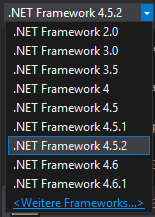
\includegraphics{Technologien_dotNetVersions}
    \caption{.NET Framework Versionen}
    \label{fig:netFramework}
\end{figure}
\justifying
\subsubsection {asp.net}
\label{sec:asp.net}
Da das Ziel der Diplomarbeit ein Webservice unter C\# ist, wurde ASP.NET verwendet. ASP.NET ist Teil des .net Frameworks, mit ihm lassen sich Webservices oder auch Webanwendungen einfach entwickeln. ASP.NET kommt bei 11.8\% aller aktiven Webseiten zum Einsatz und befindet sich deshalb auf dem 2ten Platz nach der Programmiersprache PHP. \\ \cite{aspnetstatistik} \\
\\ Im Anschluss wird durch Abbildung \ref{fig:aspNetTut01}, \ref{fig:aspNetTut02}, \ref{fig:aspNetTut03} und \ref{fig:aspNetTut04} Schritt für Schritt gezeigt wie ein ASP.NET Projekt in Visual Studio 2017 erstellt wird.
\begin{figure}[h]
    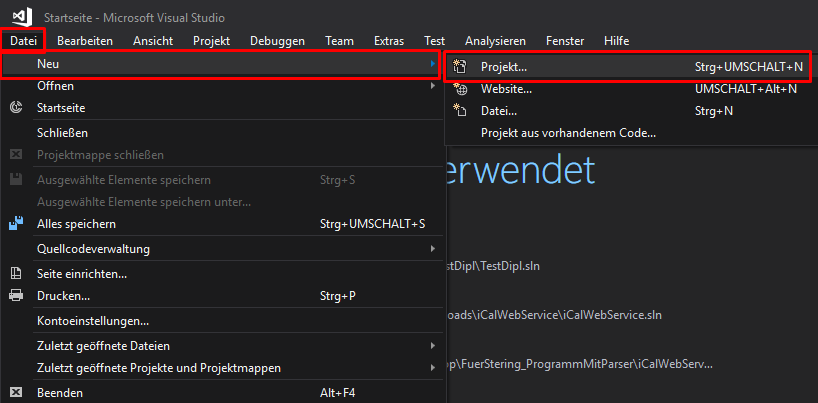
\includegraphics[width=\textwidth]{Technologien_aspNetTutorial01}
    \caption{ASP.NET Projekt erstellen}
    \label{fig:aspNetTut01}
\end{figure}
\begin{figure}[h]
    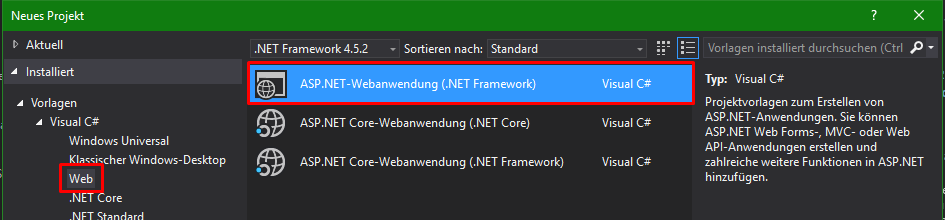
\includegraphics[width=\textwidth]{Technologien_aspNetTutorial02}
    \caption{ASP.NET Webanwendung auswählen}
    \label{fig:aspNetTut02}
\end{figure}
\begin{figure}[H]
    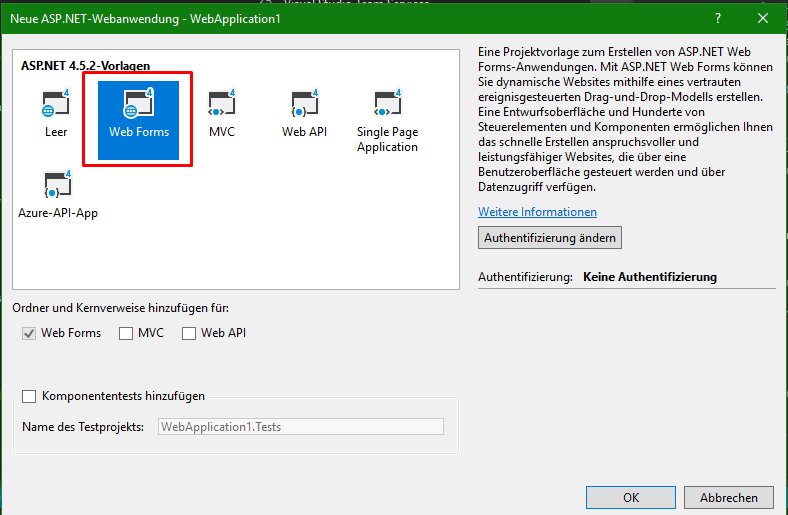
\includegraphics[width=\textwidth]{Technologien_aspNetTutorial03}
    \caption{ASP.NET Vorlage auswählen}
    \label{fig:aspNetTut03}
\end{figure}
\begin{figure}[h]
    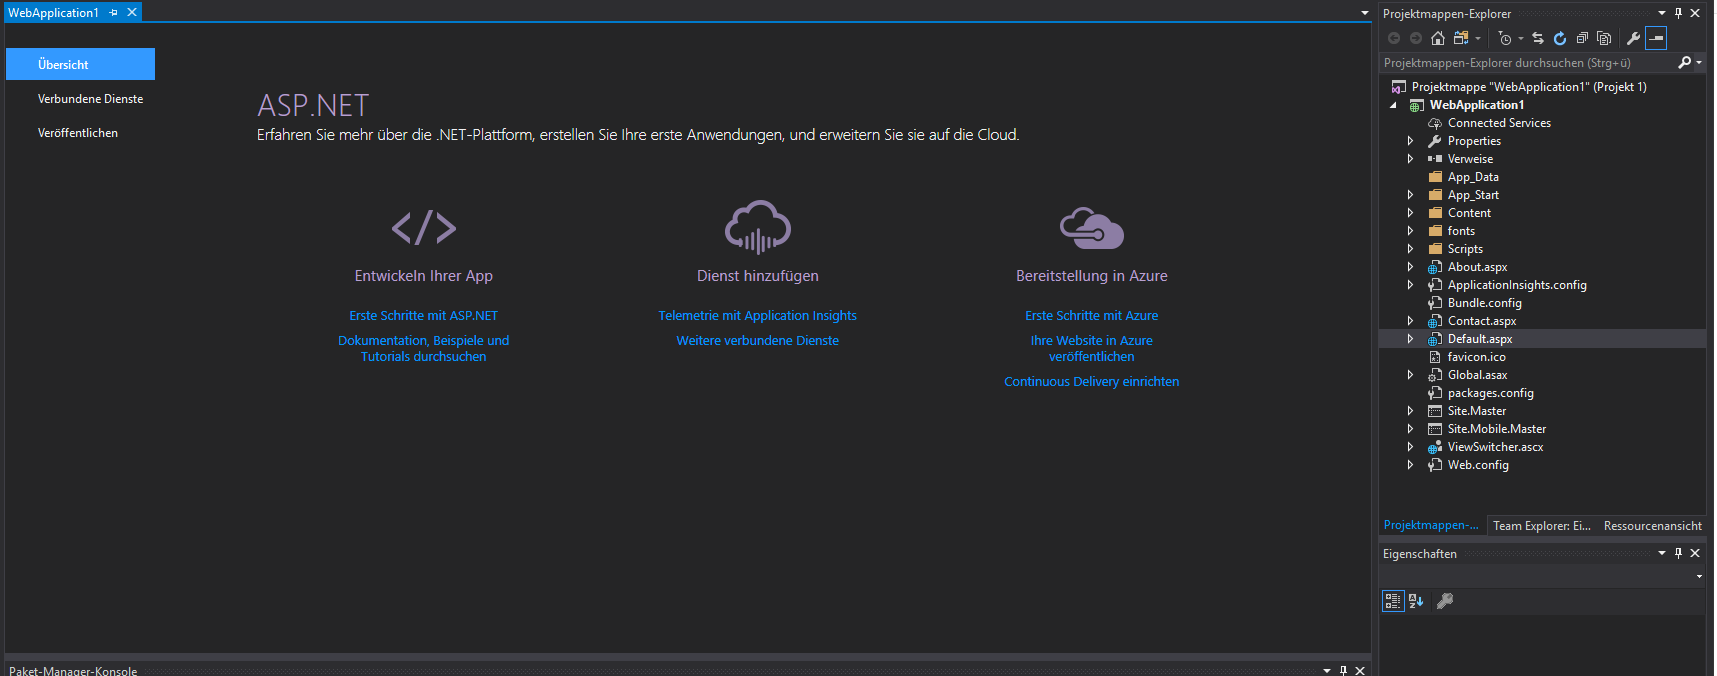
\includegraphics[width=\textwidth]{Technologien_aspNetTutorial04}
    \caption{ASP.NET Projekt Resultat}
    \label{fig:aspNetTut04}
\end{figure}
\subsubsection {MSSQL}
\label{sec:MSSQL}
MSSQL ist KEIN Teil der finalen Diplomarbeit und wurde nur zu Testzwecken verwendet. Im Laufe der Entwicklung wurde von Teammitglied Matthias Franz und Marcel Stering ein Raspberry PI als Datenbank aufgesetzt um einige Tests durchzuführen. Dies wurde mit Microsoft SQL Server verwirklicht. 
\subsubsection {Microsoft SQL Server management Studios}
\label{sec:mssql-server-management-studio}
Bei der Microsoft SQL Server entwicklung kam Microsoft SQL Server management Studios zum Einsatz, die Aufgabe des Management Studios war es den Server zu konfigurieren und zu verwalten. 
\subsubsection {Entity Framework}
\label{sec:ef}
Das Entity Framework ist ein Großteil des Projektparts "Parser". Das Entity Framework wird angewandt um den Zugriff auf die Datenbank zu erleichtern. Es dient zur objektrationalen Abbildung auf .NET Objektstrukturen. Auf die Funktionsweise des EFs wird im Kapitel ''Parser'' genauer eingegangen. \\vgl. \cite{entityframework}
%\subsubsection {iCal}
%\label{sec:ical}
%iCal ist das Format in dem ein Kalender gespeichert wird. Das Format wird unter einer eigenen Überschrift im Laufe der schriftlichen Arbeit genauer erklärt. \ref{sec:iCal}
%Ein Beispiel für den Aufbau des iCal-Formats sieht wie folgt aus: 
%\begin{flushleft}
%BEGIN:VCALENDAR \break
%   PRODID:-//ACME/DesktopCalendar//EN \break
%   METHOD:REQUEST \break
%   VERSION:2.0 \break
%   BEGIN:VEVENT \break
%   ORGANIZER:mailto:sman@netscape.com \break
%   ATTENDEE;ROLE=CHAIR;ATTSTAT=ACCEPTED:mailto:sman@netscape.com \break
%   ATTENDEE;RSVP=YES:mailto:stevesil@microsoft.com \break
%   DTSTAMP:19970611T190000Z \break
%   DTSTART:19970701T210000Z \break
%   DTEND:19970701T230000Z \break
%   SUMMARY:Phone Conference \break
%   DESCRIPTION:Please review the attached document. \break
%   UID:calsvr.example.com-873970198738777 \break
%   ATTACH:ftp://ftp.bar.com/pub/docs/foo.doc \break
%   STATUS:CONFIRMED \break
%   END:VEVENT
%\end{flushleft} \break vgl. \cite{TechnologieiCalExample}
\subsubsection {ReSharper}
\label{sec:ReSharper}
ReSharper ist eine Erweiterung für Visual Studio, welche das Entwickeln im .NET Bereich erleichtert. Die tschechische Firma JetBrains ist unter anderem Herausgeber von PyCharm, IntelliJ IDEA,  CLion und vielen weiteren hilfreichen Entwicklungs-Tools. 
\subsubsection{ReSharper Installation}
\label{sec:ReSharperInstallation}
1. ReSharper auf der JetBrains Seite unter folgendem Link herunterladen: \break \url {https://www.jetbrains.com/resharper/download/} \\
2. Nach Download, die .exe Datei ausführen \\
3. Installierte Visual Studio Version auswählen, License Agreement akzeptieren, anschließend bei gewolltem Paket auf ''Install'' klicken und auf ''Next''. 
Wenn nun auf ''Next'' geklickt wird, werden alle zu installierenden Pakete nochmal angezeigt. Falls die Auswahl passt, auf "Install" klicken. \\
4. Wenn die Installation abgeschlossen ist Fenster schließen. \\
5. Um sicherzugehen, dass die Installation erfolgt ist, Visual Studio starten. Hier sollte nun ein Fenster aufploppen um das Shortcut Scheme auszuwählen.
Wird nun eine der Möglichkeiten gewählt und die Vereinbarungen akzeptiert sollte anschließend eine Lizenz Information zu sehen sein. Hier beim Paket auf ''Start Evaluation'' klicken und anschließend auf ''OK''. ReSHarper ist nach diesen Schritten funktionsfähig und bereit zur Verwendung.
\subsubsection {PostMan}
\label{sec:PostMan}
% unzufrieden mit Formulierung
PostMan wird verwendet um API Tests durchzuführen. Die Software bietet eine sehr übersichtliche Benutzeroberfläche und ermöglicht es dem Benutzer einfach HTTP Requests zu generieren und erspart dem Anwender große Mengen an Code zu schreiben. \\
\\vgl. \cite{TechnologiePostman} \\ \break
Mithilfe von PostMan ist es möglich einfache GET-Requests zu senden, bei der Response ist mitunter möglich einzustellen wie diese angezeigt werden sollen. Auf der linken Seite der PostMan-Anwendung ist eine zeitliche Protokollierung, wann welche Anfrage gesendet wurde, sichtbar.
% HTTP und API müssen erklärt werden
\section{Kommunikation}
\label{sec:Kommunikation}
Das Kapitel Kommunikation befasst sich mit allen verwendeten Technologien, welche zur Kommunikation innerhalb des Teams verwendet wurden.
\subsubsection {Discord}
\label{sec:Discord}
Um im Laufe des praktischen Teils der Diplomarbeit die Übersicht zu behalten und alles zu organisieren wurde Discord verwendet. Discord hat viele Funktionen welche die Kommunikation im Team erleichtern. Discord bietet dem Benutzer an einen oder mehrere Server gratis zu erstellen. Ein Server kann aus Text und Sprachchannels bestehen. In einem Textchannel können festgelegte Personen schreiben und in einem Sprachchannel kann über VOIP miteinander geredet werden. Falls Teamintern etwas zu besprechen war oder Probleme auftraten bat Discord die perfekte Kommunikationsfläche. Da wir als Gruppe mehrere Projekte haben, haben wir einen "Projektserver". In diesem Projektserver wurde ein Text und Sprach Channel für die Diplomarbeit eingerichtet. Im Text Channel werden kleine Probleme, welche schnell gelöst werden können, besprochen und Files ausgetauscht. Im Sprach Channel werden gröbere Probleme besprochen oder wenn nötig Zeitplan-Änderungen behandelt. 
%Installation und Server erstellung
\subsubsection {Telegram}
\label{sec:Telegram}
Telegram wurde nicht regelmäßig verwendet, es diente als ein Backup falls Discord aus jeglichen Gründen nicht Verfügbar war. Telegram ist eine Chat-Applikation, vergleichbar mit WhatsApp. 
\section{Filesharing}
\label{sec:Filesharing}
Das Thema ''Filesharing'' ist in einer Diplomarbeit im Bereich der Software-Entwicklung essentiell. Unter dieser Überschrift werden alle Technologien im Bereich Filesharing, welche während der Diplomarbeit verwendet wurden, aufgelistet und erklärt. 
\subsubsection {TFS}
\label{sec:TFS}
Der Microsoft Team Foundation Server ist die verwendete Code-Sharing Technologie. Da der Auftraggeber, die Firma Intact GmbH oder Intact Systems, mit dieser Technologie arbeitet haben wir, bei einem der ersten Treffen, TFS für Code Sharing gewählt. Wir hatten einige Probleme mit dem TFS wodurch oft einzelne Teile des Projekts entwickelt wurden und dann in ein Projekt zusammengeführt wurden. Die Probleme waren unter anderem, dass die Firma längere Zeit gebraucht hat um den Server zur Verfügung zustellen aber auch, dass das Verbinden mit dem Server am Anfang nicht geklappt hat. 
%Anleitung wie man einen TFS benutzt ? maybe
% KORREKTUR LESEN HIER STEHEN GEBLIEBEN 
%
\subsubsection {Discord}
\label{sec:Discord}
Wie bereits bei den Technologien erwähnt haben wir auf einem Discord Server einen Text Channel eingerichtet. Dieser eignet sich nicht nur um miteinander zu schreiben sondern kann auch dafür genutzt werden mit anderen Benutzer Dateien zu teilen. 
\subsubsection {Google Drive}
\label{sec:GoogleDrive}
Google Drive ist ein von Google bereitgestellter Cloud Service um Dokumente freizugeben, Online zu bearbeiten und zu speichern.
Mithilfe von Google Drive wurde an Präsentationen und Projekten gearbeitet. Durch Google Docs und Google Präsentation fällt es leicht mit mehreren Personen gleichzeitig an einem Dokument zu arbeiten. Durch Google Drive wurden Dokumente wie die IVM Matrix, den Projektstrukturplan, die Meetings und die SCRUM Sprints erstellt und an alle Mitglieder geteilt. 
\section{Organisation}
\label{sec:Organisation}
Organisation ist ein wichtiger Teil bei einem Projekt im Team. In diesem Kapitel werden alle eingesetzten Mittel zur erleichterten Organisation aufgelistet und erklärt.
\subsubsection {Trello}
\label{sec:Trello}
Trello ist eine web-basiert Software die das Managen von Projekten vereinfacht. Trello wurde benutzt um den management Prozess Scrum erfolgreich durchzuführen. Trello bietet eine gute Übersicht über den Status des Projekts, da es Aufgaben in Form von kleinen Karten in einer Liste anzeigt. Diese Aufgaben kann mit einer verantwortlichen Person inkl. Frist versehen werden. So wird dem Scrummaster die Möglichkeit geboten 3 Listen zu erstellen: ''To Do'', ''in Arbeit'' und ''Fertig''. Je nachdem in welchem Status sich die Aufgabe befindet wird sie dementsprechend zugeteilt. \\vgl. \cite{trello} 
\section{Schriftliche Arbeit}
\label{sec:TechSchriftlicheArbeit}
Hier wird die verwendete Technologie zur Verfassung der Diplomarbeit angegeben. Mit anschließender Begründung warum sie verwendet wurde.
\subsubsection {LaTeX}
\label{sec:LaTeX}
LaTeX ist ein System mitdessen Hilfe ein Dokument erstellen werden kann. Die Formatierung dieses Dokuments läuft, anders als bei Word, über Befehle. LaTeX läuft über das Textsatzsystem TeX. TeX hat seine eigene Sprache um Formatierungen von Text oder Grafiken sehr präzise und individuell einzustellen. 
\subsubsection{Warum LaTeX?} 
\label{sec:WarumLaTeX}
Warum wurde LaTeX verwendet und nicht Word oder sonstige Programme? Sobald bei einem Dokument vorgeschriebene Formatierung einzuhalten ist oder es einen großen Umfang haben wird, lohnt es sich LaTeX zu verwenden. Mit LaTeX werden Formatierungen per Befehl definiert, am Anfang des Dokuments können gewisse Vorgaben definiert werden. So ist es möglich standardmäßige Einstellungen vorzunehmen, welche Formatierungsfehler beinahe komplett ausschließen. Nicht nur die Formatierung wird übersichtlicher und erleichtert, auch die Aufteilung des Projekts wird simpler. Es ist möglich ein Dokument als ''Haupt''-Dokument anzulegen und in diesem weitere einzelne Dokumente einzubinden. So können verschieden Themenbereiche in verschiedene Dokumente aufgeteilt werden. \\vgl. \cite{TechnologieLaTeX} 